%%%%%%%%%%%%%%%%%%%% author.tex %%%%%%%%%%%%%%%%%%%%%%%%%%%%%%%%%%%
%
% sample root file for your "contribution" to a contributed volume
%
% Use this file as a template for your own input.
%
%%%%%%%%%%%%%%%% Springer %%%%%%%%%%%%%%%%%%%%%%%%%%%%%%%%%%


% RECOMMENDED %%%%%%%%%%%%%%%%%%%%%%%%%%%%%%%%%%%%%%%%%%%%%%%%%%%
\documentclass[graybox]{svmult}



% choose options for [] as required from the list
% in the Reference Guide

\usepackage{amsmath, amssymb, mathtools, bm, xspace} % from knoblach without amsthm
\usepackage{graphicx}
\usepackage{algorithm}
\usepackage{xcolor}
%\newtheorem{theorem}{Theorem}
%\newtheorem{lemma}{Lemma}
\usepackage{dsfont}


\usepackage{mathptmx}       % selects Times Roman as basic font
\usepackage{helvet}         % selects Helvetica as sans-serif font
\usepackage{courier}        % selects Courier as typewriter font
\usepackage{type1cm}        % activate if the above 3 fonts are
                            % not available on your system
%
\usepackage{makeidx}         % allows index generation
\usepackage{graphicx}        % standard LaTeX graphics tool
                             % when including figure files
\usepackage{multicol}        % used for the two-column index
\usepackage[bottom]{footmisc}% places footnotes at page bottom

% see the list of further useful packages
% in the Reference Guide
%%%%%%%%%%%%%%%%%%%%%%%%%%
%% Mathematics
%%%%%%%%%%%%%%%%%%%%%%%%%%



% Couleurs/Style
\providecommand{\code}[1]{\textbf{\texttt{#1}}} %
\providecommand{\codeScript}[1]{\blue{\textbf{\texttt{#1}}}} %

\providecommand{\onera}[0]{\textbf{ONERA}~}
\providecommand{\dav}[0]{\textbf{Dassault-Aviation}~}
\providecommand{\airbus}[0]{\textbf{Airbus}~}
\providecommand{\edf}[0]{\textbf{EDF}~}
\providecommand{\dlr}[0]{\textbf{DLR}~}

\providecommand{\matlab}[0]{\textsc{{Matlab}}~}
\providecommand{\simulink}[0]{\textsc{{Simulink}}~}
\providecommand{\more}[0]{\textsc{\textbf{More}}~}
\providecommand{\compleib}[0]{COMPl$_e$ib~\cite{Compleib}~}
\providecommand{\rms}[0]{\textbf{RMS}~}
\providecommand{\hifi}[0]{\textbf{HiFi}~}
\providecommand{\gvt}[0]{\textbf{GVT}~}
\providecommand{\wtt}[0]{\textbf{WTT}~}
\providecommand{\wt}[0]{\textbf{WT}~}
\providecommand{\mimo}[0]{\textbf{MIMO}~}
\providecommand{\simo}[0]{\textbf{SIMO}~}
\providecommand{\miso}[0]{\textbf{MISO}~}
\providecommand{\siso}[0]{\textbf{SISO}~}
\providecommand{\dae}[0]{\textbf{DAE}~}
\providecommand{\ode}[0]{\textbf{ODE}~}
\providecommand{\lti}[0]{\textbf{LTI}~}
\providecommand{\lp}[0]{\textbf{P-LTI}~}
\providecommand{\tds}[0]{\textbf{TDS}~}
\providecommand{\lpv}[0]{\textbf{LPV}~}
\providecommand{\svd}[0]{\textbf{SVD}~} %
\providecommand{\lfr}[0]{\textbf{LFR}~}
\providecommand{\lft}[0]{\textbf{LFT}~}
\providecommand{\fft}[0]{\textbf{FFT}~}
\providecommand{\itia}[0]{\textbf{ITIA}~}
\providecommand{\irka}[0]{\textbf{IRKA}~}
\providecommand{\tfirka}[0]{\textbf{TF-IRKA}~}
\providecommand{\istia}[0]{\textbf{ISTIA}~}
\providecommand{\flistia}[0]{\textbf{FL-ISTIA}~}
\providecommand{\ietia}[0]{\textbf{IETIA}~}
\providecommand{\darpo}[0]{\textbf{DARPO}~}
\providecommand{\ioditia}[0]{\textbf{IO-dITIA}~}
\providecommand{\bt}[0]{\textbf{BT}~}
\providecommand{\tsia}[0]{\textbf{TSIA}~}
\providecommand{\loe}[0]{\textbf{Loewner}~}
\providecommand{\iloe}[0]{\textbf{iLoewner}~}
\providecommand{\ploe}[0]{\textbf{pLoewner}~}


\providecommand{\question}[1]{\red{\textbf{#1}}}
%\providecommand{\ie}[0]{\emph{i.e.}~}
%\providecommand{\etc}[0]{\emph{etc.}~}
%\providecommand{\eg}[0]{\emph{e.g.}~}
\providecommand{\ie}[0]{{i.e.}}
\providecommand{\etc}[0]{{etc.}~}
\providecommand{\eg}[0]{{e.g.}}


\definecolor{bleuONERA}{RGB}{16,97,169}
\definecolor{grisONERA}{RGB}{64,64,66}
\providecommand{\blue}[1]{\textcolor[RGB]{16,97,169}{#1}} % Bleu charte ONERA
\providecommand{\blueb}[1]{\textbf{\textcolor[RGB]{16,97,169}{#1}}} % Bleu charte ONERA
\providecommand{\grey}[1]{\textcolor[RGB]{64,64,66}{#1}} % Gris charte ONERA
\providecommand{\greyb}[1]{\textbf{\textcolor[RGB]{64,64,66}{#1}}} % Gris charte ONERA
\providecommand{\red}[1]{\textcolor[rgb]{0.98,0.00,0.00}{#1}}
\providecommand{\redb}[1]{\textbf{\textcolor[rgb]{0.98,0.00,0.00}{#1}}}
\providecommand{\green}[1]{\textcolor[rgb]{0.00,0.58,0.00}{#1}}
\providecommand{\greenb}[1]{\textbf{\textcolor[rgb]{0.00,0.58,0.00}{#1}}}

\providecommand{\orangeLight}[1]{\textcolor[rgb]{1,0.5,0}{#1}}

\providecommand{\nok}[0]{\red{$\times$}}
\providecommand{\ok}[0]{\green{$\surd$}}

% Evironnements
\newenvironment{eq}{\everymath {\displaystyle \everymath{ }} \equation}{ \endequation} %
\newenvironment{eqn}{\everymath {\displaystyle \everymath{ }\nonumber}  \equation}{ \endequation} %

% Operateurs
\DeclareMathOperator*{\argmin}{\mathbf{argmin}}
\DeclareMathOperator*{\rank}{\mathbf{rank}}
%\DeclareMathOperator*{\colspan}{\mathbf{span}}

\providecommand{\abs}[1]{\left\lvert #1 \right\rvert} %
%\providecommand{\norm}[1]{\left\lVert #1 \right\rVert} %
\providecommand{\norm}[1]{|| #1 ||} %
\providecommand{\eval}[2]{\left.#1\right\rvert_{#2}} %
\providecommand{\diag}[0]{\mathbf{diag} } %
\providecommand{\svd}[0]{\mathbf{SVD} } %
\providecommand{\im}[0]{\mathbf{Im} } %
\providecommand{\kernel}[0]{\mathbf{ker} } %
\providecommand{\trace}[0]{\mathbf{tr} } %
\providecommand{\res}[0]{\mathbf{res} } %
\providecommand{\Res}[1]{\Phi_{#1} } %
\providecommand{\det}[0]{\mathbf{det} } %
\providecommand{\ulft}[2]{\mathcal{F}_u(#1,#2)} %
\providecommand{\llft}[2]{\mathcal{F}_l(#1,#2)} %
\providecommand{\nynu}[0]{n_y\times n_u} %
\providecommand{\squarepow}[0]{\frac{1}{2}} %
\providecommand{\order}[0]{\mathbf{order}} %

\providecommand{\colspan}[1]{\mathbf{span}\left[ #1 \right]} %
\providecommand{\pare}[1]{\left(#1\right) } %
\providecommand{\tr}[1]{\trace\pare{#1} } %

% Vecteurs et systemes
\providecommand{\x}[0]{\mathbf{x}} %
\providecommand{\dx}[0]{\mathbf{\dot{x}}} %
\providecommand{\ddx}[0]{\mathbf{\ddot{x}}} %
\providecommand{\xr}[0]{\mathbf{\hat{x}}} %
\providecommand{\dxr}[0]{\mathbf{\dot{\hat{x}}}} %
\providecommand{\ddxr}[0]{\mathbf{\ddot{\hat{x}}}} %
\renewcommand{\u}{\mathbf{u}} %
\providecommand{\y}[0]{\mathbf{y}} %
\providecommand{\yr}[0]{\mathbf{\hat{y}}} %
\providecommand{\lv}[0]{\mathbf{l}} %
\providecommand{\rv}[0]{\mathbf{r}} %
\providecommand{\wv}[0]{\mathbf{w}} %
\providecommand{\vv}[0]{\mathbf{v}} %
\providecommand{\pv}[0]{\mathbf{p}} %
\providecommand{\cv}[0]{\mathbf{c}} %
\providecommand{\bv}[0]{\mathbf{b}} %

\providecommand{\Hrealr}[0]{\mathcal{\hat{S}}} %
\providecommand{\Htranr}[0]{\mathbf{\hat{H}}} %
\providecommand{\Htransr}[0]{\mathbf{\hat{H}}(s)} %
\providecommand{\Er}[0]{{\hat{E}}} %
\providecommand{\Ar}[0]{{\hat{A}}} %
\providecommand{\Br}[0]{{\hat{B}}} %
\providecommand{\Cr}[0]{{\hat{C}}} %
\providecommand{\Dr}[0]{{\hat{D}}} %

\providecommand{\Hreal}[0]{\mathcal{S}} %
\providecommand{\Htran}[0]{\mathbf{H}} %
\providecommand{\Gtran}[0]{\mathbf{G}} %
\providecommand{\Htrans}[0]{\mathbf{H}(s)} %
\providecommand{\E}[0]{{E}} %
\providecommand{\A}[0]{{A}} %
\providecommand{\B}[0]{{B}} %
\providecommand{\C}[0]{{C}} %
\providecommand{\D}[0]{{D}} %

\providecommand{\LL}[0]{{\mathds L}} %
\providecommand{\sLL}[0]{{\mathds L_\sigma}} %

% Espaces
\providecommand{\Htwo}[0]{{\mathcal{H}_{2}}} %
\providecommand{\Htwos}[0]{{\mathcal{H}_{2}^{\nynu}}} %
\providecommand{\Htwow}[0]{{\mathcal{H}_{2,\Omega}}} %
\providecommand{\Htwows}[0]{{\mathcal{H}_{2,\Omega}^{\nynu}}} %
\providecommand{\Hinf}[0]{{\mathcal{H}_{\infty}}} %
\providecommand{\Hinfs}[0]{{\mathcal{H}_{\infty}^{\nynu}}} %
\providecommand{\Hinfw}[0]{{\mathcal{H}_{\infty,\Omega}}} %
\providecommand{\Hinfws}[0]{{\mathcal{H}_{\infty,\Omega}^{\nynu}}} %
\providecommand{\Ltwo}[0]{{\mathcal{L}_{2}}} %
\providecommand{\Ltwos}[0]{{\mathcal{L}_{2}^{\nynu}}} %
\providecommand{\Ltwow}[0]{{\mathcal{L}_{2,\Omega}}} %
\providecommand{\Ltwows}[0]{{\mathcal{L}_{2,\Omega}^{\nynu}}} %
\providecommand{\Linf}[0]{{\mathcal{L}_{\infty}}} %
\providecommand{\Linfs}[0]{{\mathcal{L}_{\infty}^{\nynu}}} %
\providecommand{\Linfw}[0]{{\mathcal{L}_{\infty,\Omega}}} %
\providecommand{\Linfws}[0]{{\mathcal{L}_{\infty,\Omega}^{\nynu}}} %

\providecommand{\Cplx}[0]{\mathbb{C}} %
\providecommand{\Real}[0]{\mathbb{R}} %
\providecommand{\Nat}[0]{\mathbb{N}} %

\providecommand{\gramo}[0]{\mathcal{O}} %
\providecommand{\gramc}[0]{\mathcal{C}} %

% Matrices/Vecteurs
\providecommand{\matrixtwo}[4]{ \left[\begin{array}{cc} #1 & #2 \\ #3 & #4 \end{array}\right] } %
\providecommand{\matrixthree}[9]{ \left[\begin{array}{ccc} #1 & #2 & #3 \\ #4 & #5 & #6 \\ #7 & #8 & #9\end{array}\right] } %
\providecommand{\matrixtwocross}[4]{ \left[\begin{array}{c|c} #1 & #2 \\ \hline #3 & #4 \end{array}\right] } %
\providecommand{\matrixthreecross}[9]{ \left[\begin{array}{c|cc} #1 & #2 & #3 \\ \hline #4 & #5 & #6 \\ #7 & #8 & #9\end{array}\right] } %
\providecommand{\vectortwo}[2]{ \left[\begin{array}{c} #1 \\ #2 \end{array}\right] } %
\providecommand{\vectorthree}[3]{ \left[\begin{array}{c} #1 \\ #2 \\ #3 \end{array}\right] } %
\providecommand{\vectorfour}[4]{ \left[\begin{array}{c} #1 \\ #2 \\ #3 \\ #4 \end{array}\right] } %
\providecommand{\vectortwoT}[2]{ \left[\begin{array}{cc} #1 & #2 \end{array}\right] } %
\providecommand{\vectorthreeT}[3]{ \left[\begin{array}{ccc} #1 & #2 & #3 \end{array}\right] }%
\providecommand{\vectorfourT}[4]{ \left[\begin{array}{cccc} #1 & #2 & #3 & #4 \end{array}\right] }%
\providecommand{\vectorfiveT}[5]{ \left[\begin{array}{ccccc} #1 & #2 & #3 & #4 & #5 \end{array}\right] } %
\providecommand{\vectorfive}[5]{ \left[\begin{array}{c} #1 \\ #2 \\ #3 \\ #4 \\ #5 \end{array}\right] } 

%% Use case
%\providecommand{\useCase}[2]{
%\tikzstyle{mybox} = [draw=black, fill=blue!20, very thick, rectangle, rounded corners, inner sep=10pt, inner ysep=20pt]
%\tikzstyle{fancytitle} = [draw=black, fill=white, text=black, very thick, rounded corners]
%\begin{tikzpicture}
%\node [mybox] (box){%
%    \begin{minipage}{1\textwidth}
%        #2
%    \end{minipage}
%};
%\node[fancytitle, right=10pt] at (box.north west) {\Large #1};
%\node[fancytitle, rounded corners] at (box.east) {$\clubsuit$};
%\end{tikzpicture}
%} %


\usepackage{tikz,pgfplots,tikz-3dplot}
\usetikzlibrary{positioning, plotmarks, arrows, calc, shadings, patterns,
	decorations.pathreplacing, calc}


\makeindex             % used for the subject index
                       % please use the style svind.ist with
                       % your makeindex program

%%%%%%%%%%%%%%%%%%%%%%%%%%%%%%%%%%%%%%%%%%%%%%%%%%%%%%%%%%%%%%%%%%%%%%%%%%%%%%%%%%%%%%%%%

\begin{document}

\title*{Stability Assessment of a Two Degree of Freedom Gust Load Alleviation System}
% Use \titlerunning{Short Title} for an abbreviated version of
% your contribution title if the original one is too long
\author{Daniel Ossmann and Charles Poussot-Vassal}
% Use \authorrunning{Short Title} for an abbreviated version of
% your contribution title if the original one is too long
\institute{Dr. Daniel Ossmann \at Institute of System Dynamics and Control, German Aerospace Center, Muenchener Strasse 20, 82234 Wessling, Germany, \email{daniel.ossmann@dlr.de}
\and Dr. Charles Poussot-Vassal \at Systems and Signal Processing Department, ONERA Centre de Toulouse, 2 Avenue Edouard Belin, 31000 Toulouse, France \email{Charles.Poussot-Vassal@onera.fr}}
%
% Use the package "url.sty" to avoid
% problems with special characters
% used in your e-mail or web address
%
\maketitle


%\abstract*{Each chapter should be preceded by an abstract (10--15 lines long) that summarizes the content. The abstract will appear \textit{online} at \url{www.SpringerLink.com} and be available with unrestricted access. This allows unregistered users to read the abstract as a teaser for the complete chapter. As a general rule the abstracts will not appear in the printed version of your book unless it is the style of your particular book or that of the series to which your book belongs. Please use the 'starred' version of the new Springer \texttt{abstract} command for typesetting the text of the online abstracts (cf. source file of this chapter template \texttt{abstract}) and include them with the source files of your manuscript. Use the plain \texttt{abstract} command if the abstract is also to appear in the printed version of the book.}

\abstract*{	In this paper a novel approach to design linear disturbance estimator is presented. The linear approach relies on the idea of directly decoupling everything but the disturbance input from the estimate by using advanced nullspace computation techniques. The main advantage of the approach is that disturbance estimators of minimal order, using available and numerically reliable tools, can be designed. The approach is applied to a generic model of a business jet aircraft. The derived disturbance estimate is used in a control algorithm to reduce the wing bending moments on the aircraft in case of wind gusts.
Both, the disturbance estimator together with the load alleviation controller are verified in a non-linear closed loop aircraft simulation model.}

\abstract{	In this paper a novel approach to design linear disturbance estimator is presented. The linear approach relies on the idea of directly decoupling everything but the disturbance input from the estimate by using advanced nullspace computation techniques. The main advantage of the approach is that disturbance estimators of minimal order, using available and numerically reliable tools, can be designed. The approach is applied to a generic model of a business jet aircraft. The derived disturbance estimate is used in a control algorithm to reduce the wing bending moments on the aircraft in case of wind gusts. Both, the disturbance estimator together with the load alleviation controller are verified in a non-linear closed loop aircraft simulation model.}



\section{INTRODUCTION}
Estimating an unknown disturbance using linear observers and estimators can be  powerful in conjunction with feedback control \cite{Franklin02}. The idea is to appropriately include a disturbance estimate in the control law so that disturbance effects can be approximately removed. This requires the estimation of the disturbance with high accuracy. There is a long history on disturbance estimator design and thus a rich literature available on different design methods. 
The simplest design idea arises in the frequency domain, where the known, disturbance free plant model is used to derive the difference between the measured and estimated output, which is considered to be the disturbance. See for example references  \cite{Schrijver02, hori92} for description and proper applications. 
The unknown input observer \cite{Hostetter73, Basile69, Gourishangkar77} translates the problem into the time and state-space domain and estimates both the systems states and the disturbance. This  requires the definition of disturbance dynamics to allow the disturbance estimation via  a dedicated system state.
The problem formulation in the time domain and the introduction of disturbance states also opened the door to the adaption of well developed state estimators as Kalman filters or  $\mathcal{H}_\infty$-norm based filter designs for the disturbance estimation problem
\cite{Wang04}. The similarity of the Kalman filter and the classical designs in the frequency domain are discussed in \cite{Schrijvert00}.


%There is also a broad literature on non-linear disturbance observer design methods \cite{Chen04}. These, however, are outside of scope of this paper .

% Ein wenig Fehlerdetektion
The topic of disturbance estimators is closely related to the approaches used in the fault detection and isolation (FDI) community. Interpreting the appearing faults as disturbances, a lot of approaches available in the FDI literature can be used for the estimation of disturbances. The main difference between FDI and disturbance estimation is, that the disturbance observer has to accurately reflect the disturbance input signal while FDI aims to generate \textit{any} signal which is decoupled from all known and unknown inputs but the fault(s) to be detected. However, some approaches can be adapted to not only provide fault detection but also fault estimation, \ie, reflecting the actual value of the fault. This fault estimation problem is comparable to the disturbance estimation problem and methods used for the one can be used for the other. Notable linear design methods to solve  FDI problem are Luenberger observers \cite{Jones71} and Luenberger-type approaches using for example geometric methods \cite{Massoumnia86} or eigenstructure assignment \cite{Chen99}.
Further, also arising from the idea of disturbance observers, unknown input observers \cite{Chen99} are well established in the field of FDI.
Beside the observer based approaches, parity space  methods \cite{Chow84, Lou86} and nullspace based approaches have been introduced, see \eg, \cite{frisk_01,varga07}. These two methods allow the design of detectors of minimal order. The minimal order characteristics of the observer reduce the dependence on the underlying model dynamics and thereby increases implicitly the robustness to modeling errors and model uncertainties.
The main difference in the two mentioned approaches lies in the computational and numerical manner in solving the decoupling conditions. The nullspace based design methods can be considered to be numerically more reliable \cite{Var09}. 

% In this paper
In this paper we make use of the latest developments in the nullspace based design methods in the FDI community to present a novel approach for the design of disturbance estimators.
Originally developed to solve FDI problems \cite{frisk_01, Varga17}, the disturbance estimation problem is stated herein in a form, which allows its direct solving  via the idea of nullspace computations.
The design methodology  to design a minimal order disturbance estimator is introduced in section \ref{sec:th}. 
In case of design models with very high state dimension, which are for example usually present when dealing with load alleviation problems on aircraft, an a priori model reduction is recommended. Thus, in section \ref{sec:mr} an advanced model approximation technique is additionally discussed to facilitate the minimal order estimator design.
A main focus of the paper lies on the realistic and  industrially relevant  application. In section \ref{sec:app} a generic example of a medium size business jet is introduced. It serves as basis for the order reduction and the subsequent disturbance observer design. The model is further utilized in section \ref{sec:res} to verify the load alleviation capabilities  of the proposed load alleviation system.
The idea of this load alleviation system is to use the wind estimate to trigger a dedicated feedback law which alleviates the maximum bending moments on the wings in case of increased wind gusts. A description of this non-linear control law is provided in section \ref{sec:app}.C.
%For the design a lower order, linear model needs to be derived. Advanced model reduction techniques are discussed which allow the sophisticated reduction and derive models, which are suitable for the observer design algorithms. 


\section{Model approximation}\label{sec:mr}

When dealing with industrial problems such as aircraft systems, associated models usually embed unsteady aerodynamics as well as structural modes and aerodynamical delays. Consequently, the dimension of the  state-space dimensions can be very large, and additionally models can include delays and potentially mixing differential and algebraic equations. Thus, before the methods presented in section \ref{sec:th} can be applied, a pre-processing step, to reduce the state dimension and simplify the complexity should be first applied in order to improve the numerical treatment and accuracy of the results. A short reminder of the methods involved in section \ref{sec:app} are briefly discussed in this section. As these methods are not the main topic of this paper, more details on infinite or data-driven model approximation can be found in \cite{AntoulasSurvey:2016,DalmasECC:2016,Meyer:2016} and on finite order large-scale model approximation in \cite{AntoulasBook:2005,GugercinSIAM:2008}.  Let us follow these two classes of problems and remind the driving ideas as follows.

\subsection{Infinite  dimensional or data-driven model approximation}\label{sec:app_a}

%Given an infinite dimensional model $\Htran$, it is possible to obtain the  frequency-domain responses $\mathbf{\Phi}_i \in \mathds C^{n_y \times n_u}$ for different frequency samples $\omega_i$ ($i = 1, \dots , N$). Then, one can write $\Htran(\imath \omega_i) = \mathbf{\Phi}_i$. One of the data-driven approach is based on the interpolatory framework well defined in \cite{Mayo:2007,AntoulasSurvey:2016}, involving the Loewner matrices. The method consists of an \emph{exact rational model interpolation}, optionally followed by a \emph{reduction procedure}. To this aim, let us first partition the collected data $(\omega_i,\mathbf{\Phi}_i)_{i=1}^N$ in two disjoint sets as follows ($N=q+k$):
%\begin{eq}
%	\begin{array}{rcl}
%		\imath [\omega_1,\dots , \omega_N] &=& [\mu_1, \dots , \mu_{q}] \cup [\lambda_1, \dots , \lambda_{k}] \\ ~
%		[\mathbf{\Phi}_1,\dots , \mathbf{\Phi}_N] &=& [\tilde{\vv}_1,\dots , \tilde{\vv}_{q}] \cup [\tilde{\wv}_1, \dots , \tilde{\wv}_{k}].
%	\end{array}
%\end{eq} 
Given an infinite dimensional model $H$, it is possible to obtain the  frequency-domain responses ${\Phi}_i \in \mathds C^{n_y \times n_u}$ for different frequency samples $\omega_i$ ($i = 1, \dots , N$). Then, one can write $H(\imath \omega_i) = {\Phi}_i$. One of the data-driven approach is based on the interpolation framework well defined in \cite{Mayo:2007,AntoulasSurvey:2016}, involving the Loewner matrices. The method consists of an \emph{exact rational model interpolation}, optionally followed by a \emph{reduction procedure}. To this aim, let us first partition the collected data $(\omega_i,{\Phi}_i)_{i=1}^N$ in two disjoint sets as follows ($N=q+k$):
\begin{eq}
	\begin{array}{rcl}
		\imath [\omega_1,\dots , \omega_N] &=& [\mu_1, \dots , \mu_{q}] \cup [\lambda_1, \dots , \lambda_{k}] \\ ~
		[{\Phi}_1,\dots , {\Phi}_N] &=& [\tilde{v}_1,\dots , \tilde{v}_{q}] \cup [\tilde{w}_1, \dots , \tilde{w}_{k}].
	\end{array}
\end{eq} 
%Then, define $\lv_j \in \mathds C^{n_y\times 1}$ ($j=1,\dots , q$) and $\rv_i \in \mathds C^{n_u\times 1}$ ($i=1,\dots , k$) the $q$ left and $k$ right tangential directions. Using these tangential directions, let us define $\vv_j^*=\lv_j^*\tilde{\vv}_j \in \mathds C^{1\times n_u}$ and $\wv_i=\tilde{\wv}_i\mathbf r_i \in \mathds C^{n_y\times 1}$ the \emph{left} and \emph{right tangential} data directions, respectively. Based on the left interpolation driving frequencies $\{\mu_i\}_{i=1}^q \in \Cplx$ with left output or tangential directions $\{\lv_i\}_{i=1}^q \in \Cplx^{n_y}$, producing the left responses $\{\vv_i\}_{i=1}^q$ and right interpolation driving frequencies $\{\lambda_i\}_{i=1}^k \in \Cplx$ with right input or tangential directions $\{\rv_i\}_{i=1}^k \in \Cplx^{n_u}$, producing the right responses $\{\wv_i\}_{i=1}^k$, the objective is to find a model transfer function $\Htran$ which is a tangential interpolant of the data, \ie satisfies the following left and right interpolation conditions:
Then, define $l_j \in \mathds C^{n_y\times 1}$ ($j=1,\dots , q$) and $r_i \in \mathds C^{n_u\times 1}$ ($i=1,\dots , k$) the $q$ left and $k$ right tangential directions. Using these tangential directions, let us define $v_j^*=l_j^*\tilde{v}_j \in \mathds C^{1\times n_u}$ and $w_i=\tilde{w}_i r_i \in \mathds C^{n_y\times 1}$ the \emph{left} and \emph{right tangential} data directions, respectively. Based on the left interpolation driving frequencies $\{\mu_i\}_{i=1}^q \in \Cplx$ with left output or tangential directions $\{l_i\}_{i=1}^q \in \Cplx^{n_y}$, producing the left responses $\{v_i\}_{i=1}^q$ and right interpolation driving frequencies $\{\lambda_i\}_{i=1}^k \in \Cplx$ with right input or tangential directions $\{r_i\}_{i=1}^k \in \Cplx^{n_u}$, producing the right responses $\{w_i\}_{i=1}^k$, the objective is to find a model transfer function $\tilde H$ which is a tangential interpolant of the data, \ie, satisfies the following left and right interpolation conditions:
%\begin{eq}
%	\left.
%	\begin{array}{c}
%		\lv_j^*\Htran(\mu_j) = \vv_j^* \\
%		\text{for $j=1,\dots, q$}
%	\end{array}
%	\text{~~and~~}
%	\begin{array}{c}
%		\Htran(\lambda_i)\rv_i = \wv_i \\
%		\text{for $i=1,\dots, k$}
%	\end{array}
%	\right\}.
%	\label{eq:interpContrain}
%\end{eq}
\begin{eq}
	\left.
	\begin{array}{c}
		l_j^*\tilde H(\mu_j) = v_j^* \\
		\text{for $j=1,\dots, q$}
	\end{array}
	\text{~~and~~}
	\begin{array}{c}
		\tilde H(\lambda_i)r_i = w_i \\
		\text{for $i=1,\dots, k$}
	\end{array}
	\right\}.
	\label{eq:interpContrain}
\end{eq}
%
%
The interpolation problem \eqref{eq:interpContrain} can be solved thanks to the Loewner framework (see, \eg, \cite{Mayo:2007}). One of the important property of the Loewner approach is that it encodes the minimal McMillian degree of the interpolation model and its minimal realization order $n$. This then leads to an exact descriptor model interpolating the data, especially useful, when the number of data is very large.

\subsection{Finite dimensional model approximation}\label{sec:app_b}
Once an exact interpolation model $\tilde H$ has been obtained, with potentially large dimension, a second step then consists in approximating this finite order model with a low dimensional one. One common objective in model approximation consists in finding a reduced-order model that well captures the main original input/output dynamical behavior. To address this objective, the (frequency-limited) $\mathcal{H}_2$-norm mismatch error is commonly used, see \eg, \cite{GugercinSIAM:2008,VuilleminPhD:2014}. The resulting approximation problem consists thus in seeking a low order approximation model $\hat H(s)$ of $\tilde H(s)$, such that:
%\begin{eq}
%	\Htranr := \arg \min_{
%		\small
%		%\begin{array}{c}
%		\mathbf G\in\mathcal H_2^{n_y\times n_u} \  \rank(\mathbf G)=r \ll n
%		%\end{array}
%		\normalsize
%	} ||\Htran-\mathbf G||_{\mathcal{H}_{2} \text{ or } \mathcal{H}_{2,\Omega}}.
%	\label{pb:h2}
%\end{eq}
\begin{eq}
	\hat H := \arg \min_{
		\small
		\begin{array}{c}
			G\in\mathcal H_2^{n_y\times n_u} \\  \text{rank}(G)=r \ll n
		\end{array}
		\normalsize
	} ||\tilde H-G||_{\mathcal{H}_{2}}.
	\label{pb:h2}
\end{eq}

Beside the fact that problem \eqref{pb:h2} is non convex and non-linear, some conditions have been proposed to reach the so-called \emph{first order optimality conditions} and procedures to ensure that a local (hopefully global) optimum is reached. Moreover, the proposed IRKA and FL-ISTIA algorithms are appropriate to practically tackle these problems (see \eg, \cite{GugercinSIAM:2008,VuilleminPhD:2014} for details). %As  emphasized by the following theorem and corollary, this optimum can be reached thanks to interpolatory methods \cite{GugercinSIAM:2008}. %Let briefly recall and discuss the main results, stated for MIMO LTI DAE models, as follows.
Finally, the derived  model $\hat H$ can be easily brought into the form (\ref{eq:sys}) by separating the inputs accordingly.


\section{Stability Assessment}\label{sec:st}






\section{Disturbance estimator design}\label{sec:th}
In this section the disturbance estimator design problem is generally derived. It is shown how it is connected to the idea of nullspace computations for linear dynamical systems. 

\subsection{Problem formulation}
Consider the linear model described by the input-output form
\begin{equation}\label{eq:sys}
	y(s) = G_u(s) u(s) + G_{\bar d} \bar d(s)  + G_d d(s),
\end{equation}
where $y(s)$, $u(s)$, and $\bar d(s)$  are the Laplace-transformed
vectors of the $p$-dimensional system output vector $y(t)$, the $m_u$-dimensional control input vector $u(t)$, and the $m_{\bar d}$-dimensional disturbance vector $\bar d(t)$, respectively. $d(s)$ is the Laplace-transformed of scalar  disturbance input $d(t)$ to be estimated.
$G_u(s)$, $G_{\bar d}(s)$, and $G_d(s)$ are the transfer-function matrices (TFMs) from
control inputs to  outputs, disturbance inputs to outputs, and disturbance input to be estimated  to outputs, respectively. Note that only one disturbance $d(s)$ out of the full disturbance vector $[ \bar d(s) \; d(s)]^T$ shall be estimated.  Thus, a disturbance estimate $\tilde d(s)$ needs to be decoupled from any additional disturbances $\bar d(s)$ acting on the system. This is no restriction to the design process as for $N_d = m_{\bar d} + m_d$ disturbances acting on the system, $N_d$ individual estimators can be designed using the methods described below, if the according design conditions are fulfilled.

For the system described in (\ref{eq:sys}) a linear disturbance estimator processes the measurable system outputs $y(t)$ and control inputs $u(t)$ and generates the disturbance estimate $\tilde d(t)$. In the input-output form this can be described by
\begin{equation}\label{eq:est}
	\tilde d(s) = O(s)
	\begin{bmatrix}
		y(s) \\ u(s)
	\end{bmatrix},
\end{equation}
where $O(s)$ is the TFM of the disturbance estimator. For a physically realizable
disturbance estimator, $O(s)$ must be proper and stable. The order of $O(s)$ is the dimension of the state vector of a minimal state-space realization of $O(s)$. 
The general description in (\ref{eq:est}) allows the definition of the disturbance estimation problem (DEP):

Design a physically realizable linear disturbance estimator of the form (\ref{eq:est}) such that for all $u(t)$ and $\bar d(t)$ 
\begin{equation*}
	\begin{array}{ll}
		(i) & \tilde d(t) = 0 \text{ when } d(t) = 0 \\ 
		(ii) &\tilde d(t) \approx d(t) \text{ when } d(t) \neq 0 \\ 
		(iii) & \tilde d(t) \text{ is asymptotically bounded.}
	\end{array}
\end{equation*}
Additionally, $O(s)$ shall be of minimal order ($iv$). 


\subsection{Solving the DEP}
The requirements ($i$) and ($ii$) of the DEP are easily transformed into  algebraic conditions. Therefore, the system's input-output equation (\ref{eq:sys}) is inserted in the disturbance estimator equation (\ref{eq:est}), so that the disturbance estimate depends on the control and disturbance inputs, \ie,
\begin{equation}\label{eq:full}
	\tilde d(s) = O(s) 
	\begin{bmatrix}
		G_u(s) & G_{\bar d}(s) & G_d(s) \\ I_{m_u}& 0 & 0
	\end{bmatrix}
	\begin{bmatrix}
		u(s) \\ \bar d(s) \\ d(s)
	\end{bmatrix}.
\end{equation}
The decoupling condition $(i)$ requires that the disturbance estimate $\tilde d(s)$ is decoupled from all inputs $u(s)$ and disturbances $\bar d(s)$, which shall not be estimated. This is equivalent of demanding 
\begin{equation}\label{eq:nr}
	O(s) 
	\begin{bmatrix}
		G_u(s) & G_{\bar d}(s)  \\ I_{m_u}& 0
	\end{bmatrix}
	:= O(s) G_e(s) =  0
\end{equation}
%In words, the disturbance observer $O(s)$ has to be designed, that all inputs $u(s)$ and disturbances $\bar d(s)$ are decoupled from the disturbance estimate $\tilde d(s)$.
It follows that $O(s)$ needs to be a left annihilator of $G_e(s)$. 
By deriving a minimal basis $N_l(s)$ for the left nullspace of $G_e(s)$,  the design conditions $(i)$ can be tackled. 
For design condition $(ii)$, the basic constraint
\begin{equation}\label{eq:con}
	O(s) 
	\begin{bmatrix}
		G_{d}(s)  \\  0
	\end{bmatrix}
	\neq  0
\end{equation}
must be fulfilled. This can only be achieved, if the DEP is actually solvable. The solve-ability condition follows the theorem presented in \cite{Var09}:

\begin{theorem}
	For the system (\ref{eq:sys}) the DEP is solvable if and only if
	\begin{equation}\label{eq:cond}
		\text{rank}\left( 
		\begin{bmatrix}
			G_{\bar d}(s)  &  G_{d}(s) 
		\end{bmatrix} \right)
		>
		\text{rank} 
		(G_{\bar d}(s)).
	\end{equation}
\end{theorem}
\vspace{+3mm}
Thus, the disturbance to be estimated needs to be linearly independent of all the other disturbances. Note that the condition (\ref{eq:cond}) is independent of the control input $u$. Thus, for the case $m_{\bar d} = 0$, the DEP is always solvable. This makes sense as just known inputs and one unknown  input to be estimated act on the system.

If condition (\ref{eq:cond}) is fulfilled, a disturbance observer fulfilling ($ii$) which is stable ($iii$) as well as proper and minimal (iv)  can be constructed by linear combination of the rows of the left nullspace basis $N_l(s)$ of the $G_e(s)$ \cite{Var09}, \ie,
\begin{equation}\label{eq:par}
	O(s) = h(s) N_l(s).
\end{equation}
Note that any linear combination of $N_l(s)$ solves the design condition $(i)$ but it has to be checked if (\ref{eq:con}) is ensured to fulfill condition ($ii$).
To solve the DEP herein, the transfer function vector is defined as $h(s) = k w(s)$, which consists of a transfer function vector $w(s)$  to make the filter proper, stable and of least order. The constant  $k$ is used for scaling to ensure a transfer behavior from $d$ to $\tilde d$ of 1. If the DEP is solvable, it is always possible to freely select the scaling $k$. 
As $k$ is selected to be a constant scalar herein, its value is chosen based on the transfer gain from the disturbance input to the derived disturbance estimator output at a certain frequency. Note that this does usually not restrict the tracking of the disturbance to a single frequency, as disturbances often show constant gain over a wider frequency range. More details on the actual computation are presented next.


\subsection{Computation}
The  expression (\ref{eq:par}) represents a parametrization of all possible disturbance estimators and is the basis of the so-called nullspace based filter design methods. These methods have been formally introduced in \cite{frisk_01} using polynomial basis and extended to be numerically more reliable algorithms in \cite{varga07, Var09} using rational basis, both for fault detection purposes. Successful applications of the approaches can be found in \cite{ossmann15c,VOss_13a,Ossmann17}. 

The slightly modified computation procedure to compute a disturbance estimator  using these methods herein can be summarized in three dedicated steps. If condition (\ref{eq:cond})  is fulfilled, 
\begin{equation*}
	\begin{array}{ll}
		(I.) & \text{compute a minimal left nullspace basis } N_l(s)  \\
		&  \text{of } G_e(s), \\
		(II.) & \text{compute a rational vector } w(s) \text{ such that } \tilde O(s)= \\
		&  w(s) N_l(s) \text{ is proper, stable, has least order, } \\
		&   \text{and (\ref{eq:con}) is fulfilled,} \\
		(III.) & \text{select a constant } k \text{ such that }   O(s) = k W(s) N_l(s)  \\ 
		&  \text{ensures a transfer from } d \text{ to } \tilde d \text{ of } 1 \text{ at a defined} \\ & \text{frequency.}\\
	\end{array}
\end{equation*}
For steps ($I$.) and ($II$.) we rely on the numerically sound approach presented in \cite{varga06}. It allows to derive a  rational nullspace basis allowing to generate a minimal, proper and stable disturbance observer $\tilde O(s)$. In more detail, step ($I$.) is solved using matrix pencil methods. The minimal order in ($II$.) is then ensured via solving a minimum dynamic cover problem and the stable and proper dynamics are achieved via a QR decomposition. Interested readers in the computational ideas and their details are referred to \cite{Varga17}.

One essential difference to the fault detection problem is the requirement that in case of a disturbance estimator the estimator's output shall reflect the disturbance magnitude. This is required  as this estimate is usually directly used as input signal in a feedback controller. Thus, to allow the fault estimation  the correct scaling of the observer ($III$.) needs to be explicitly considered.
If the DEP is solvable, condition (\ref{eq:nr}) holds for any observer $\tilde O(s)$ derived via  (\ref{eq:par}). Thus, equation (\ref{eq:full}) reduces to
\begin{equation}
	\tilde d(s) = 
	\begin{bmatrix}
		\tilde O_y(s) & \tilde O_u(s) 
	\end{bmatrix}
	\begin{bmatrix}
		y(s) \\ u(s)
	\end{bmatrix}  =  \tilde O_y(s) G_{ d}(s)  d(s),
\end{equation}
where $\tilde O(s)  = [\tilde O_y(s) \,\, \tilde O_u(s) ]$ is separated into $\tilde O_y(s)$, which processes the system measurements $y$, and into $\tilde O_u(s)$, which processes the (known) control inputs $u$.
Note that $\tilde O_y(s) G_{ d}(s)$ is one single-input single-output transfer function as only scalar disturbances $d$ are considered in (\ref{eq:sys}). Thus, considering the requirement that the magnitude of $\tilde d$ follows $d$ and moving into the frequency domain, leads to 
\begin{equation}
	k |\tilde O_y(\imath \omega) G_{d}(\imath \omega)|  = 1.
\end{equation}
To follow the disturbance signal $d$ at a desired  frequency $\omega_d$, the scaling for the disturbance observer $O(s)$ can be selected as $k  = |\tilde O_y(\imath \omega_d) G_{d}(\imath \omega_d)|^{-1}$.
As an example, if the steady state value of the disturbance estimate shall equal the steady state value of the disturbance, $\omega_d = 0$ is an appropriate choice. As the dynamics of the  disturbance observer can be freely chosen \cite{Varga17}, the ensuring of a small lag between the disturbance its estimate can be ensured via setting adequately fast disturbance observer dynamics.

The presented approach herein and the available algorithms allow the reliable and efficient design of disturbance estimator up for reasonable sized systems. If large models are given, model reduction is recommended before to the estimator design. 





\section{Application}\label{sec:app}
Reducing structural loads on an aircraft by advanced control techniques is a main research interest of today's aircraft industry. Reducing the loads allows building a lighter aircraft and thereby  saves costs. The loads arise from steering the aircraft (maneuver loads) and from external disturbance inputs, (gust loads). The latter are considered in this paper for a generic business jet aircraft.

For being able to realistically compute and compare loads with  and without load alleviation controller, while taking into account as much as possible structural interactions, an aircraft model with about  300 states  is available. The model includes detailed structural and aerodynamic effects, delays, realistic actuator and sensor models as well as a baseline control law, providing adequate handling qualities to the pilot.
The control inputs to the open loop aircraft model are the  commands of the elevator, the inner ailerons and the outer ailerons. 
The gust impact on the model is characterized by  nine inputs describing the position, velocity and acceleration impact at three different locations along the fuselage.
As measured signals for feedback control, the pitch rate, the load factor  and the angle of attack are provided.
The provided baseline controller only commands the elevator while  the load alleviation controller shall use the ailerons symmetrically to alleviate the bending moments due to gusts.

The open loop model, i.e., without baseline controller, serves as basis for the disturbance observer design. The design will be carried out for a fixed aircraft speed and altitude as an example and verified in the full non-linear, closed loop aircraft model including a case with varying mass and center of gravity position.

\subsection{Model approximation}
The high number of states as well as the nine disturbance inputs makes the 
estimator and control design challenging. Thus the idea is to reduce the state dimension and the number  of disturbance inputs. In view of disturbance estimator and control design, it is preferable to use a single disturbance single input.

The nine disturbance inputs are  actually used to model a \textit{single} gust hitting  three different parts  (front, middle, rear) of the aircraft one after another. The derivatives of the three gust input positions are required to consider the unsteady aerodynamics. 
Consequently, the second and third set of gust inputs are equal to the first one but delayed by a fixed time delay. Thus, mathematically the second and third set of inputs can be derived by simply delaying the first on. Additionally, the velocity and acceleration of the first gust input can be derived by derivative action on the first gust input position, finally reducing the gust inputs to a single one.
%After these modifications, the resulting model now embeds two internal delays (denoted $\tau_1$ and $\tau_2$, related to the velocity of the aircraft and patch where the gust is impacting the fuselage) and have a rank deflective descriptor form. These internal delays are explained by the use of exact delay actions applied on the exact derivative terms. As a consequence, at this stage, the linear time-invariant dynamical system can be represented by a first order descriptor realization with $n_u$ inputs (one signle gust niput), $n_y$ outputs, $n$ internal variables and two internal delays. The model is given by a set of differential and algebraic equations (\textbf{DAE}) where states are described by $\E\dx(t) =\A_0 \x(t) + \A_1 \x(t-\tau_1)+ \A_2 \x(t-\tau_2) +\B \u(t)$ (with $\E$ rank deflective) and outputs $\y(t) = \C \x(t)$, where, $\x(t) \in \Real^{n} := \mathcal X$ is the internal variables, and $\u(t) \in \Real^{n_u} := \mathcal U$ and $\y(t) \in \Real^{n_y} := \mathcal Y$ are the input, output functions, respectively, while $\E,\A_0,\A_1,\A_2 \in \mathds{R}^{n \times n}$, $\B \in \mathds{R}^{n\times n_u}$ and $\C \in \mathds{R}^{n_y \times n}$ are constant matrices. The matrix pencil is regular if the matrix $(\A_0 +\A_1e^{-\tau_1\lambda}+\A_2e^{-\tau_1\lambda}) - \lambda\E$ is non-singular for some finite $\lambda \in \Cplx$ and a $\{\tau_1,\tau_2\}$ couple. In this case, the associated transfer function is
After these modifications, the resulting model now embeds two internal delays (denoted $\tau_1$ and $\tau_2$, related to the velocity of the aircraft) and has a rank deflective descriptor form. These internal delays are explained by the use of exact delay actions applied on the exact derivative terms. Thus, the linear time-invariant dynamical system can be represented by a first order descriptor realization with $n_u$ inputs (including one single gust input), $n_y$ outputs, $n_x$ internal variables, and the two internal delays. The model is given by a set of differential and algebraic equations 
\begin{eq}
	\begin{array}{rcl}
		\E \dot x(t) &=&\A_0 x(t) + \A_1 x(t-\tau_1)+ \A_2 x(t-\tau_2) +\B u(t)\\
		y(t) &=& \C x(t),
	\end{array}
\end{eq}
with the  rank defective matrix $\E$,  the internal variables
$x(t) \in \Real^{n_x} := \mathcal X$, and the the input and output functions $u(t) \in \Real^{n_u} := \mathcal U$ and $y(t) \in \Real^{n_y} := \mathcal Y$, respectively. $\E,\A_0,\A_1,\A_2 \in \mathds{R}^{n_x \times n_x}$, $\B \in \mathds{R}^{n_x \times n_u}$ and $\C \in \mathds{R}^{n_y \times n_x}$ are constant matrices. The matrix pencil is regular if the matrix $(\A_0 +\A_1e^{-\tau_1\lambda}+\A_2e^{-\tau_1\lambda}) - \lambda\E$ is non-singular for some finite $\lambda \in \Cplx$ and a $\{\tau_1,\tau_2\}$ couple. In this case, the associated transfer function is
\begin{eq}
	H(s) = \C\big(s\E-\A_0-\A_1e^{-\tau_1s}-\A_2e^{-\tau_2s}\big)^{-1}\B+\D.
\end{eq}
Obviously, due to the presence of delays in the dynamical part of the equations, the resulting model is now of infinite dimension. To cope with this,  first  an exact stable Loewner interpolation of this infinite model by a finite order one is performed as discussed in section \ref{sec:app_a}. This leads to a large scale descriptor model of dimension $n$, which exactly interpolates the infinite dimensional model $H$, with $\tilde{H}(s)$, of the form
\begin{eq}
	\tilde{H}(s) = \tilde{\C}\big(s\tilde{\E}-\tilde{\A}\big)^{-1}\tilde{\B}.
\end{eq}
Now, this finite order model (\eg with a finite number of eigenvalues) can be readily approximated using any (frequency-limited) $\mathcal H_2$ oriented model approximation techniques as discussed in section \ref{sec:app_b} and further presented in \eg, \cite{GugercinSIAM:2008,VuilleminSSSC:2013,PoussotMORE:2012}. This leads to a reduced order model with dimension $r\ll n$, as, 
\begin{eq}
	\hat H(s) = \Cr\big(s\Er-\Ar\big)^{-1}\Br
\end{eq}
which minimizes the (frequency-limited)  mismatch error. 
Finally, the aircraft model of about 300 states with nine disturbance inputs has been approximated with a model of order $r=25$ with a single disturbance input. This reduced model can now be used to design the disturbance estimator. 
%Importantly, readers should note that the presented order reduction approach allows transforming an infinite descriptor model equipped with a large state-space vector into a finite order one with a reduced state-space vector dimension.

\subsection{Estimator Design}
A disturbance estimator with the presented methods in section \ref{sec:th} is designed for the aircraft. The final design model after the model approximation features 25 states, three control inputs, namely elevator, symmetric inner aileron and symmetric outer aileron position, one gust input and the two measurable outputs, \ie,  pitch rate and the load factor. Applying the approach presented in section \ref{sec:th} results in a first order disturbance estimator. As the dynamics of the detector can be freely chosen, the single real pole is set to -1.
This value still provides an adequate estimation delay and ensures reasonable estimator gains.
The resulting state-space representation of the disturbance estimator is given by
\begin{equation}\label{eq:obs}
	\begin{array}{rcr}
		\dot x_e  &=& -x_e + B_e
		\begin{bmatrix}
			q & n_z & \eta & \xi_i & \xi _o 
		\end{bmatrix}^T \,\,\, \vspace{+1mm} \\ 
		\tilde d &=&  x_e + 
		D_e
		\begin{bmatrix}
			q & n_z & \eta & \xi_i & \xi _o 
		\end{bmatrix}^T,
	\end{array}
\end{equation}



\subsection{Control Strategy}
Having an estimate of the gust available, a non-linear control strategy is developed. When a gust hits the aircraft, the increased angle of attack on the wings leads to an increased  lift  on the wings. This lift increases the encountered wing bending moment. The idea is to symmetrically and rapidly deflect the ailerons, so that the additional lift resulting from the wind gust gets reduced. If the disturbance estimate exceeds a defined threshold value, the ailerons are deflected, where the direction of the deflection depends on the gust direction. This direction is determined from the change in the (sensed) angle of attack $\alpha$. The proposed control law is a bang-bang like controller with a threshold based triggering. The threshold dis selected based on simulations.
The controller stays active as long the gust estimate exceeds its threshold but at least one second after activation to avoid a rapid on and off switching.

\begin{figure}[bth]
	\centering
	\usetikzlibrary{positioning,plotmarks, matrix, arrows, calc, shapes}
\tikzstyle{blockdiag}	= [node distance=5mm, >=stealth', semithick]
\tikzstyle{block}			= [draw, rectangle, minimum width=1.05cm, minimum
height=.8cm]


\tikzstyle{block2}			= [draw, rectangle, minimum width=1.05cm, minimum
height=.8cm, fill=white]

\tikzstyle{sum} = [draw,circle,inner sep=0pt, minimum size=6pt]
\tikzstyle{connector} = [draw,circle,inner sep=0pt, minimum size=0.001pt, 
fill=black]
\tikzstyle{connector2} = [draw,circle,inner sep=0pt, minimum size=2pt, 
fill=black]
\tikzstyle{gain} = [draw,regular polygon, regular polygon 	sides=3,thick,minimum height=3em,minimum width=4em, rotate=30]
\tikzstyle{bguide} = [rectangle,minimum height=3em,minimum	width=4em]
\tikzstyle{line} = [thick]
\tikzstyle{branch} = [circle,inner sep=0pt,minimum size=1mm,fill=black,draw=black]
\tikzstyle{guide} = [anchor=center]

\pgfdeclarelayer{bg}    % declare background layer
\pgfsetlayers{bg,main}

\begin{tikzpicture}[blockdiag, auto, scale=0.8]

% Blocks
\node[block,minimum width=1.25cm, minimum height=1.5cm](Plant) {$G$};
\node[block, minimum width=1.25cm, minimum height=1cm,left=of Plant, xshift=-1.5cm, yshift=0.47cm] (C) {$C_\eta$};
\node[block, minimum width=1.25cm, minimum height=1cm,below=of Plant,  yshift=0cm] (Obsv) {\textcolor{blue}{$O_e$}};
%\node[block, minimum width=1cm, minimum height=.8cm,below=of Obsv,  yshift=-0.2cm] (logic) {$> \tau_{th}$};
\node[block2, minimum width=1.25cm, minimum height=1cm,left=of Obsv, xshift=-1.5cm, yshift=0.5cm] (Cload) {\textcolor{blue}{$C_{\Delta \xi}$}};


\node[connector2, right=of Plant, xshift = 0.65cm] (con1) {}; 
\node[connector2, right=of Plant, xshift = 0.25cm, yshift = 0.5cm] (con2) {}; 
\node[connector2, right=of Cload, xshift = 0.65cm, yshift = -0.23cm] (con3) {}; 
\node[connector2, right=of Cload, xshift = 0.25cm, yshift = 0.25cm] (con4) {}; 
\node[connector2, right=of C, xshift = 1cm] (con5) {}; 
\node[connector, below=of Cload, xshift = -0.5cm, yshift = 0.2cm] (con6) {}; 
\node[connector, above=of Cload, xshift = 0.5cm, yshift = -0.2cm] (con7) {}; 
\node[connector, right=of Plant, xshift = 0.1cm, yshift = -0.5cm] (con8) {}; 
\node[connector, below=of Obsv, xshift = 0cm, yshift = -0.0cm] (con9) {}; 

\draw[->]  (Plant.east) ++(0cm,0.6cm)  --  ++(1cm,0cm) node[pos=0.27,yshift=-1mm] {$q$} --  ++(0cm,1.60cm)  -| ($(C.north)+(0.4cm,0cm)$);
\draw[->]  (Plant.east) ++(0cm,0cm)  --  ++(1.5cm,0cm) node[pos=0.27,yshift=-1mm] {$n_z$}  --  ++(0cm,2.60cm)   -|  ($(C.north)-(0.4cm,0cm)$);

\draw[->]  (Cload.east) ++(0cm,0.3cm)  --  ++(1.0cm,0cm) node[pos=0.39,yshift=-.5mm] {\textcolor{blue}{$\Delta \xi_i$}}    |- ($(Plant.west)+(0cm,0cm)$);
\draw[->]  (Cload.east) ++(0cm,-0.3cm)  --  ++(1.5cm,0cm) node[pos=0.29,yshift=-.5mm] {\textcolor{blue}{$\Delta  \xi_o$}}    |- ($(Plant.west)+(0cm,-0.6cm)$);

\draw[->]  (C)  --  ($(Plant.west)+(0cm,0.59cm)$)node[pos=0.13]{$\eta$};
\draw[->]   (con9) -| (Cload.south);
\draw[<-, color=red] (Plant.north) -- +(0cm, +1cm)node[left, pos=.7]{\textcolor{red}{$d$}};

\draw[->]  (con1)  |-  ($(Obsv.east)+(0cm,-0.5cm)$);
\draw[->]  (con2)  |-  ($(Obsv.east)+(0cm,0cm)$);
\draw[->]  (con8)  |-  ($(Obsv.east)+(0cm,+0.5cm)$);


\draw[->]  (con5)  |-  ($(Obsv.west)+(0cm,0.5cm)$);
\draw[->]  (con4)  |-  ($(Obsv.west)+(0cm,0cm)$);
\draw[->]  (con3)  |-  ($(Obsv.west)+(0cm,-0.5cm)$);


\draw[-]  (con9)  --  (Obsv)node[pos=0.75,yshift=-1mm] {\textcolor{blue}{$\tilde d$}};
\draw[-]  (Plant.east)++(0cm,-0.625cm)   --  (con8)node[pos=0.4,yshift=-.5mm] {$\alpha$};
%\draw[->]  (con8)  -- ++(0.0cm,-4.5cm)  -- ++(-8.5cm,0cm)  |-  (Cload.west);

;\end{tikzpicture} 
	\caption{Closed loop structure including aircraft dynamics, baseline controller, disturbance observer with triggering logic, and  load alleviation controller. }
	\label{fig:cl}	
\end{figure}

The overall structure of the closed loop system is depicted in Fig. \ref{fig:cl}. The baseline controller $C_\eta$ uses the measurements load factor $n_z$ and the pitch rate $q$ from the aircraft $AC$ as inputs to generate the elevator deflection $\eta$. It ensures adequate handling and disturbance rejection in the longitudinal, rigid body motion of the aircraft. The disturbances $d$ are acting on the aircraft as unknown inputs. The aircraft in this illustration also includes the sensor and actuator dynamics.
If the gust estimate $\tilde d$ of the estimator $O_e$ is above the defined threshold $\tau_{\text{th}}$, the load alleviation is triggered via the Boolean variable $i$. The angle of attack $\alpha$ is used to determine the direction of the load alleviation aileron command.



\section{Closed loop load verification}\label{sec:res}


\section{CONCLUSIONS}
In this paper an approach to design linear disturbance estimators of minimal order using the nullspace based design technique as well as advanced model approximation techniques has been presented. The proposed method has been successfully applied to a generic business jet aircraft model. Based on the estimated disturbance a simple control strategy has been employed to reduce the maximum wing bending moments encountered due to wind gusts.








\section*{Conclusions}




\begin{acknowledgement}
This work has been funded within the frame of the Joint Technology
Initiative JTI Clean Sky 2, AIRFRAME Integrated Technology Demonstrator
platform "AIRFRAME ITD" (contract N$^\circ$ CSJU-CS2-GAM-AIR-2014-15-01 Annex
1, Issue B04, October 2nd, 2015) being part of the Horizon 2020 research
and Innovation framework program of the European Commission.
\end{acknowledgement}
%
%\section*{Appendix}
%\addcontentsline{toc}{section}{Appendix}

\bibliographystyle{spmpsci}
\bibliography{BIB_Ossmann,_biblioCPV,_biblioPoussot}
%\printbibliography

%\input{referenc}
\end{document}

%%%%%%%%%%%%%%%%%%%%%%%%%%%%%%%%%%%%%%%%%%%%%%%%%%%%%%%%%%%%%%%%%%%%%%%%%%%%%%%%%%%%%%%%%%%%%%%%%%%%%%%%%%%%%%%%%%%%%%%%%%%%


%\begin{figure}[t]
%	\sidecaption[t]
%	% Use the relevant command for your figure-insertion program
%	% to insert the figure file.
%	% For example, with the option graphics use
%	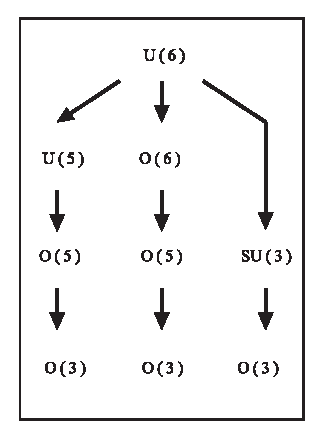
\includegraphics[scale=.65]{figure}
%	%
%	% If no graphics program available, insert a blank space i.e. use
%	%\picplace{5cm}{2cm} % Give the correct figure height and width in cm
%	%
%	%\caption{Please write your figure caption here}
%	\caption{If the width of the figure is less than 7.8 cm use the \texttt{sidecapion} command to flush the caption on the left side of the page. If the figure is positioned at the top of the page, align the sidecaption with the top of the figure -- to achieve this you simply need to use the optional argument \texttt{[t]} with the \texttt{sidecaption} command}
%	\label{fig:2}       % Give a unique label
%\end{figure}


%\begin{table}
%	\caption{Please write your table caption here}
%	\label{tab:1}       % Give a unique label
	%
%\begin{tabular}{p{2cm}p{2.4cm}p{2cm}p{4.9cm}}
%	\hline\noalign{\smallskip}
%	Classes & Subclass & Length & Action Mechanism  \\
%	\noalign{\smallskip}\svhline\noalign{\smallskip}
%	Translation & mRNA$^a$  & 22 (19--25) & Translation repression, mRNA cleavage\\
%	Translation & mRNA cleavage & 21 & mRNA cleavage\\
%	Translation & mRNA  & 21--22 & mRNA cleavage\\
%	Translation & mRNA  & 24--26 & Histone and DNA Modification\\
%	\noalign{\smallskip}\hline\noalign{\smallskip}
%\end{tabular}
%$^a$ Table foot note (with superscript)
%\end{table}


%\begin{svgraybox}
%If you want to emphasize complete paragraphs of texts we recommend to use the newly defined Springer class option \verb|graybox| and the newly defined environment \verb|svgraybox|. This will produce a 15 percent screened box 'behind' your text.
%
%If you want to emphasize complete paragraphs of texts we recommend to use the newly defined Springer class option and environment \verb|svgraybox|. This will produce a 15 percent screened box 'behind' your text.
%\end{svgraybox}


%
%\begin{proof}
%\smartqed
%Proof text goes here.
%\qed
%\end{proof}

%If you want to list definitions or the like we recommend to use the Springer-enhanced \verb|description| environment -- it will automatically render Springer's preferred layout.
%
%\begin{description}[Type 1]
%	\item[Type 1]{That addresses central themes pertainng to migration, health, and disease. In Sect.~\ref{sec:1}, Wilson discusses the role of human migration in infectious disease distributions and patterns.}
%	\item[Type 2]{That addresses central themes pertainng to migration, health, and disease. In Sect.~\ref{subsec:2}, Wilson discusses the role of human migration in infectious disease distributions and patterns.}
%\end{description}

%
